\chapter{Suggestions to Improve The Existing System} \label{suggestions}

\section{System Perspective}
Improved FarmBot includes a Mobile Application and ForumBot. The Mobile Application brings farm management to mobile devices, while ForumBot allows users to exchange farming tips and layouts. These new features integrate seamlessly with the existing system, enhancing the user experience with additional flexibility and community support.

% Improved Context Diagram
\begin{figure}[htbp]
    \centering
    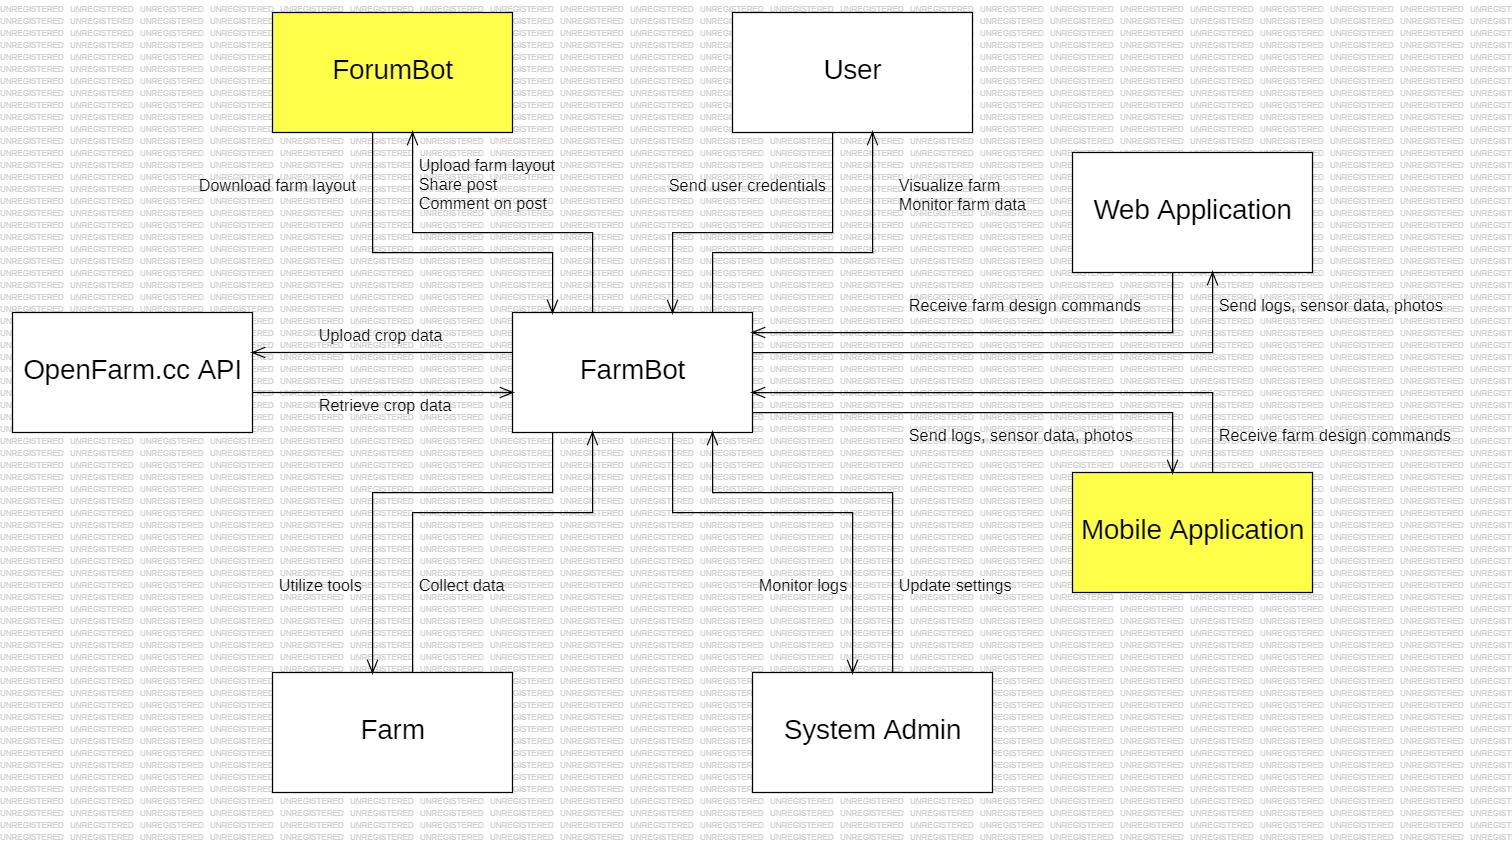
\includegraphics[width=1\linewidth]{Figures/context_diagram_improved.jpg}
    \caption{Context Diagram of the Improved System}
    \label{ContextDiagramImproved}
\end{figure}

\newpage

\section{External Interfaces}
In addition to the external interfaces represented in 3.1, Mobile Application and ForumBot are introduced. Each of them has its own external interface:
\begin{itemize}
    \item \textbf{Mobile Application Interface:} This interface manages the interactions between the user's mobile device and FarmBot. It supports user authentication, task scheduling, and retrieval of data such as sensor readings and hardware information. It's tailored for mobile usage, taking into account the device's name and the user's phone number for personalized interactions.
    \item \textbf{ForumBot Interface:} This interface is designed for community engagement within the FarmBot ecosystem. It allows users to create a username and password, post discussions, share insights, comment on existing posts, and manage their profile and activity logs. Users can also download and upload farm layouts, making it a platform for sharing knowledge and farming strategies.
\end{itemize}

% Improved External Interfaces Diagram
\begin{figure}[htbp]
    \centering
    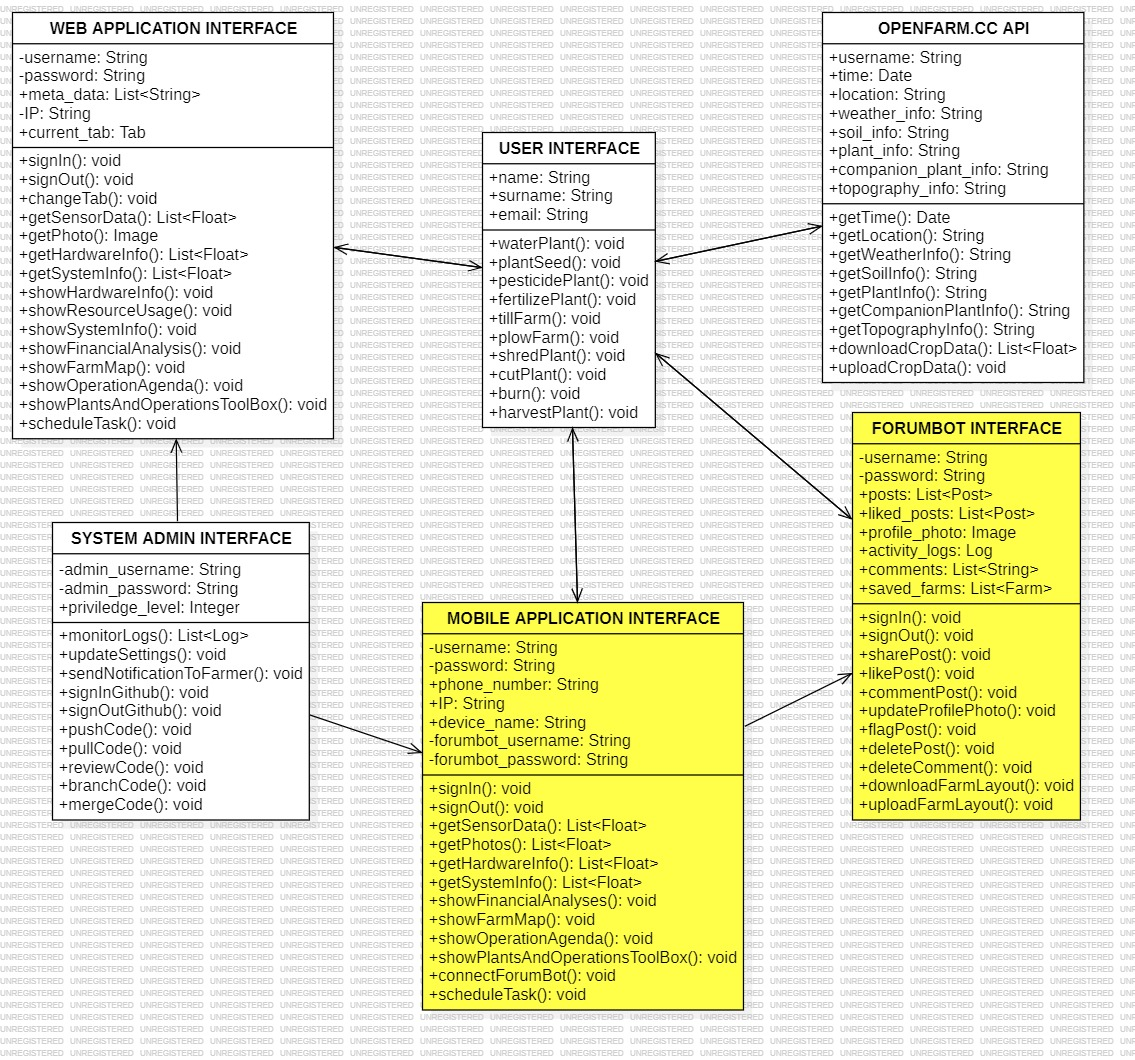
\includegraphics[width=1\linewidth]{Figures/external_interfaces_improved.jpg}
    \caption{External Interfaces of the Improved System}
    \label{ExternalInterfacesImproved}
\end{figure}

\newpage

\section{Functions}
The improved use case diagram integrates new external entities, which are Mobile Application and ForumBot. Now, users can engage with the FarmBot community by sharing and commenting on posts and downloading farm layouts from ForumBot. The Mobile Application enables users to schedule watering tasks directly from their mobile devices, enhancing FarmBot's accessibility and ease of use. These new use cases are pivotal for a more interactive and mobile-friendly FarmBot experience.

% Improved Use Case Diagram
\begin{figure}[htbp]
    \centering
    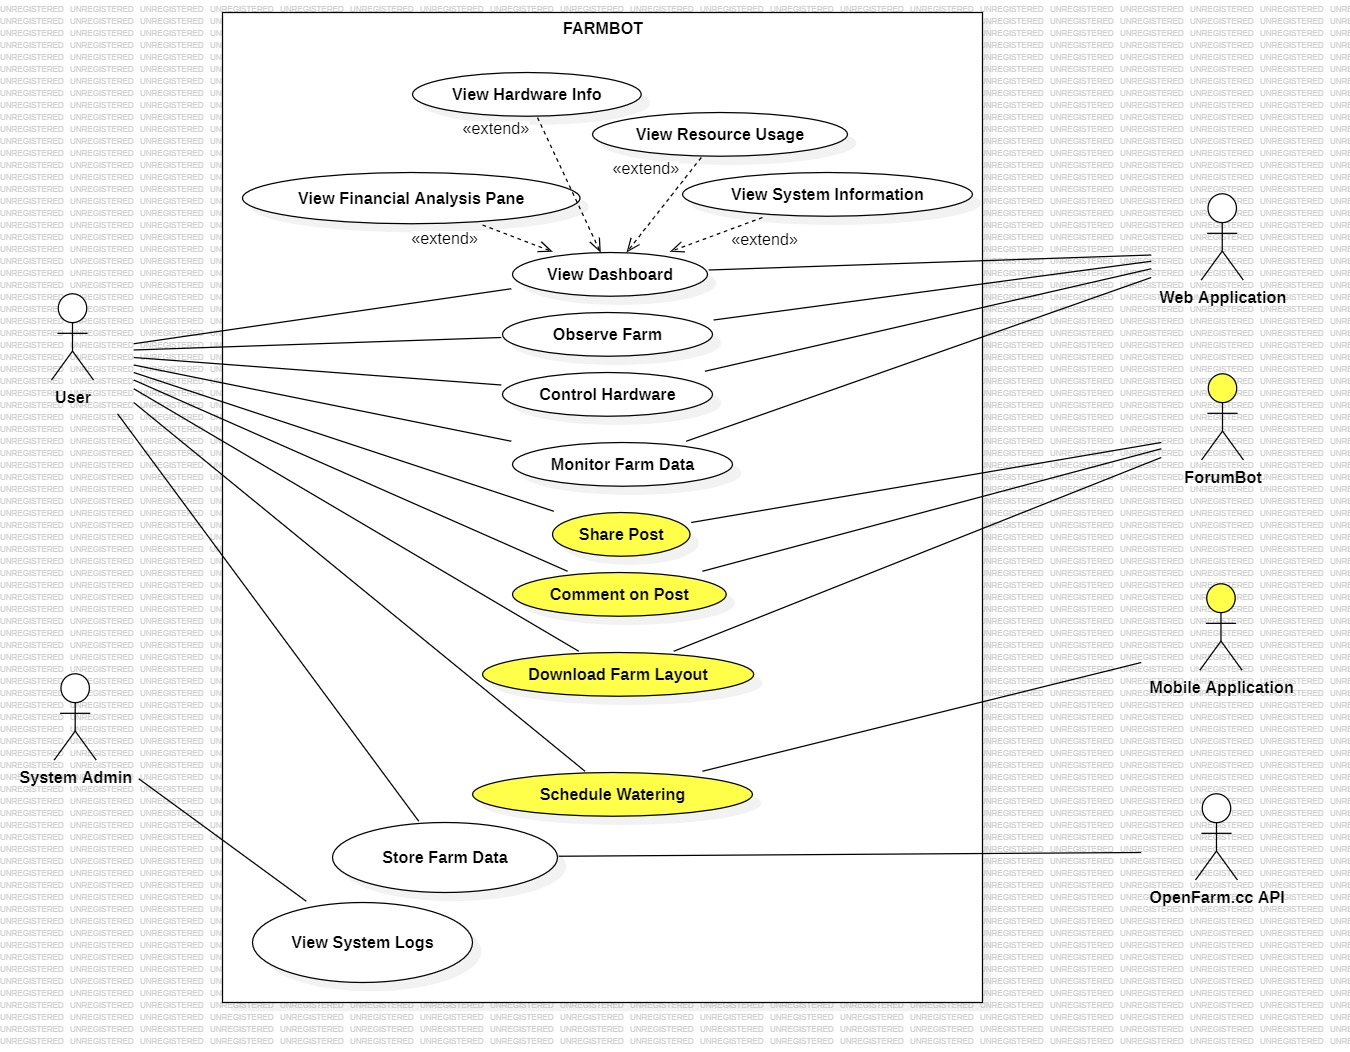
\includegraphics[width=1\linewidth]{Figures/use_case_diagram_improved.jpg}
    \caption{Use Case Diagram of the Improved System}
    \label{UseCaseImproved}
\end{figure}

\newpage

% Download Farm Layout Use Case Table
\begin{longtblr}
[
 caption = {Tabular Description of the \textbf{Download Farm Layout} Use Case of the Improved System},
 label = {DownloadFarmLayout}
]
{
  colspec = {|X|X|},
  hlines
}
\textbf{Use Case Name} & Download Farm Layout \\ \hline
\textbf{Actors} & User, ForumBot \\ \hline
\textbf{Description} &  The user downloads a farm layout shared by another user from ForumBot, a platform for sharing and downloading FarmBot farm layouts. \\ \hline
\textbf{Preconditions} & The user must be registered and logged into ForumBot.  \\ \hline
\textbf{Data} & Farm layout files including plant placement, watering schedules, and other operational sequences. \\ \hline
\textbf{Response} & The user successfully downloads the selected farm layout to their local device. \\ \hline
\textbf{Stimulus} & The user selects a farm layout and initiates the download process on ForumBot. \\ \hline
\textbf{Normal Flow} & {
1. User logs into ForumBot website.\\
2. User browses farm layouts available on ForumBot.\\
3. User selects a desired farm layout.\\
4. User clicks the download button for the selected layout.\\
5. ForumBot processes the request and initiates the file download.\\
6. The farm layout file is downloaded to the user's local device.
} \\ \hline
\textbf{Alternative Flow} & If the desired farm layout is not available or the download link is broken, the user can request the layout directly from the layout's author via a messaging feature on ForumBot. \\ \hline
\textbf{Exception Flow} & If the user is not logged in or the session has expired, they are redirected to the login page. \\ \hline
\textbf{Post Conditions} &  The selected farm layout is stored on the user's local device, ready for upload to their FarmBot Web Application. \\ \hline
\textbf{Comments} & This use case enables users to leverage community-shared farm layouts, fostering a collaborative environment where users can learn from and improve upon each other's designs. It emphasizes the importance of user interaction and content sharing within the FarmBot community.
\end{longtblr}

% Download Farm Layout Activity Diagram
\begin{figure}[htbp]
    \centering
    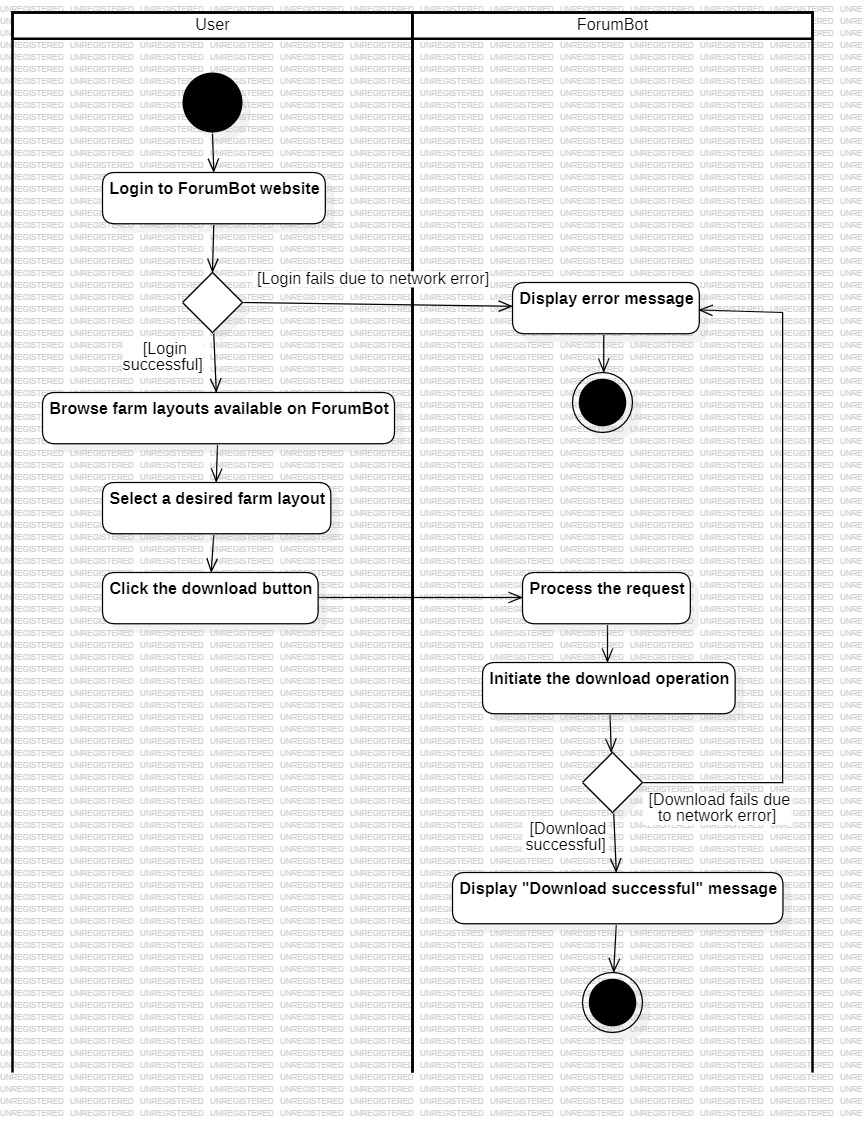
\includegraphics[width=1\linewidth]{Figures/download_farm_layout_activity_diagram.jpg}
    \caption{Activity Diagram for \textbf{Download Farm Layout} Use Case of the Improved System}
    \label{DownloadFarmLayoutActivityDiagram}
\end{figure}

\newpage

% Share Post Use Case Table
\begin{longtblr}
[
 caption = {Tabular Description of the \textbf{Share Post} Use Case of the Improved System},
 label = {SharePost}
]
{
  colspec = {|X|X|},
  hlines
}
\textbf{Use Case Name} & Share Post \\ \hline
\textbf{Actors} & User, ForumBot \\ \hline
\textbf{Description} & The User shares a post on ForumBot, a community platform where FarmBot users can share insights, ask questions, and discuss various topics related to FarmBot. \\ \hline
\textbf{Preconditions} & The user must be registered and logged into ForumBot.  \\ \hline
\textbf{Data} & Text content, images, or links included in the post. \\ \hline
\textbf{Response} &  The post is successfully published on ForumBot, visible to other users. \\ \hline
\textbf{Stimulus} & The user composes a post and submits it for publication on ForumBot. \\ \hline
\textbf{Normal Flow} & {
1. User logs into ForumBot and clicks to the "Create Post" button.\\
2. User composes the post and attaches any relevant images or links.\\
3. User submits the post.\\
4. ForumBot processes the submission and publishes the post.\\
5. The post becomes visible to other ForumBot users in the relevant discussion category.
} \\ \hline
\textbf{Alternative Flow} & - \\ \hline
\textbf{Exception Flow} & If the user is not logged in or the session has expired, they are redirected to the login page. \\ \hline
\textbf{Post Conditions} & The user's post is publicly accessible on ForumBot, facilitating community engagement and information exchange. \\ \hline
\textbf{Comments} & This use case fosters an active community dialogue, allowing users to contribute knowledge, share experiences, and support one another in the effective use of FarmBot.
\end{longtblr}

% Share Post State Diagram
\begin{figure}[htbp]
    \centering
    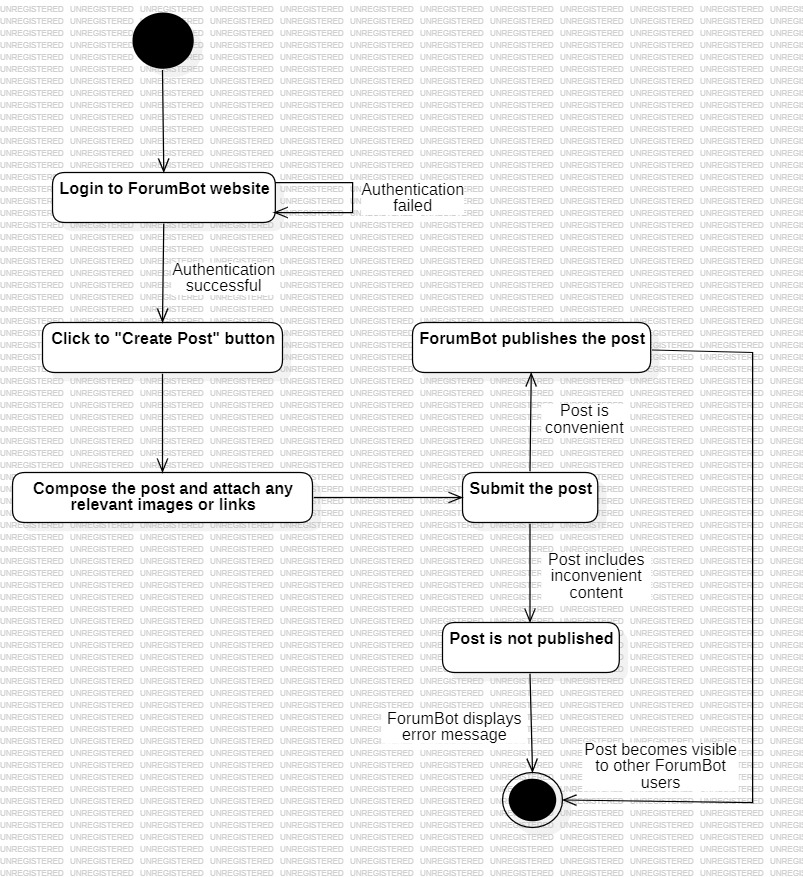
\includegraphics[width=1\linewidth]{Figures/share_post_state_diagram.jpg}
    \caption{State Diagram for \textbf{Share Post} Use Case of the Improved System}
    \label{SharePostStateDiagram}
\end{figure}

\newpage

% Comment on Post Use Case Table
\begin{longtblr}
[
 caption = {Tabular Description of the \textbf{Comment on Post} Use Case of the Improved System},
 label = {CommentOnPost}
]
{
  colspec = {|X|X|},
  hlines
}
\textbf{Use Case Name} & Comment on Post \\ \hline
\textbf{Actors} & User, ForumBot \\ \hline
\textbf{Description} &  The User submits a comment on an existing post within the ForumBot platform. \\ \hline
\textbf{Preconditions} & The user must be registered and logged into ForumBot.  \\ \hline
\textbf{Data} & Text content, images, or links included in the comment. \\ \hline
\textbf{Response} & The user's comment is successfully added below the original post, visible to other users. \\ \hline
\textbf{Stimulus} & The user decides to contribute to a discussion by commenting on a post on ForumBot. \\ \hline
\textbf{Normal Flow} & {
1. User logs into ForumBot and navigates to a post of interest.\\
2. User enters their comment in the designated comment section below the post.\\
3. ForumBot processes the submission and displays the comment under the post.\\
4. ForumBot processes the submission and publishes the post.\\
5. The comment becomes visible to other ForumBot users, facilitating further discussion.
} \\ \hline
\textbf{Alternative Flow} & - \\ \hline
\textbf{Exception Flow} & If the user is not logged in or the session has expired, they are redirected to the login page. If the user attempts to submit an empty comment or one that violates community guidelines, ForumBot displays an error message. \\ \hline
\textbf{Post Conditions} &  The user's comment is publicly accessible on ForumBot, contributing to the ongoing dialogue and community engagement around the post. \\ \hline
\textbf{Comments} & This use case encourages active participation and exchange of ideas within the FarmBot community, enabling users to ask questions, provide answers, and share insights, thereby enriching the collective knowledge base.
\end{longtblr}

% Schedule Watering Use Case Table
\begin{longtblr}
[
 caption = {Tabular Description of the \textbf{Schedule Watering} Use Case of the Improved System},
 label = {ScheduleWatering}
]
{
  colspec = {|X|X|},
  hlines
}
\textbf{Use Case Name} & Schedule Watering \\ \hline
\textbf{Actors} & User, Mobile Application \\ \hline
\textbf{Description} & The user schedules a watering operation for their FarmBot via the Mobile Application, setting up the timing and duration for watering specific plant zones. \\ \hline
\textbf{Preconditions} & The user must be registered with and logged into the Mobile Application linked to their FarmBot. \\ \hline
\textbf{Data} & Specific zones to be watered, start time, duration of watering. \\ \hline
\textbf{Response} &  The Mobile Application schedules the watering operation on the FarmBot, and the user receives confirmation of the scheduled task. \\ \hline
\textbf{Stimulus} & The user decides to schedule a watering operation through the Mobile Application. \\ \hline
\textbf{Normal Flow} & {
1. User logs into the Mobile Application.\\
2. User navigates to the "Schedule Task" and then the "Watering Schedule" section.\\
3. User selects the plant zones to water, sets the start time, and specifies the duration.\\
4. User confirms and submits the watering schedule.\\
5. Mobile Application sends the request to Raspberry Pi. \\
6. Raspberry Pi executes the scheduled watering operation in the specified time. \\
7. Raspberry Pi sends signals to Mobile Application every time the watering operation happens.\\
8. Mobile Application sends notifications to the user every time the watering operation happens.
} \\ \hline
\textbf{Alternative Flow} & - \\ \hline
\textbf{Exception Flow} & If the user is not logged in or the session has expired, they are redirected to the login page. If FarmBot is offline or unable to execute the scheduled task, the user is notified of the failure to schedule or execute the watering operation. \\ \hline
\textbf{Post Conditions} & The watering operation is successfully scheduled and confirmed, ready to be executed by FarmBot at the specified time. \\ \hline
\textbf{Comments} & This use case enables precise and efficient water management, allowing users to optimize watering schedules based on the specific needs of their plants, thereby conserving water and ensuring plant health.
\end{longtblr}

% Schedule Watering Sequence Diagram
\begin{figure}[htbp]
    \centering
    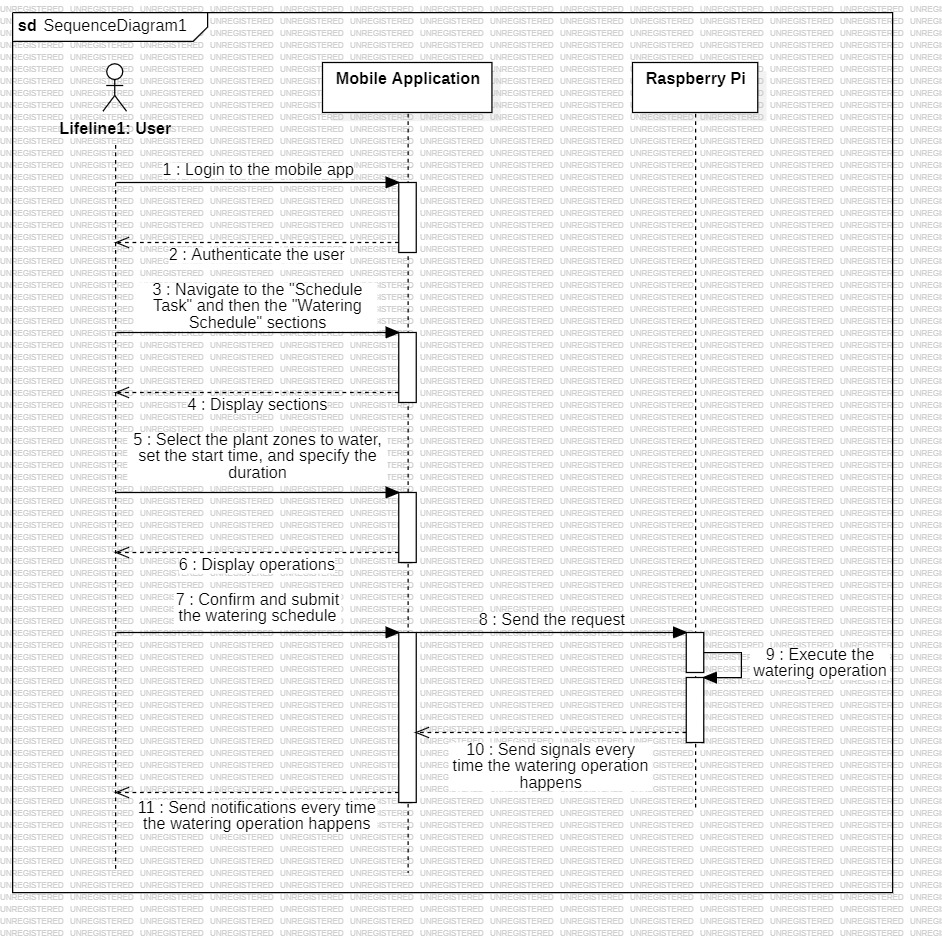
\includegraphics[width=1\linewidth]{Figures/schedule_watering_sequence_diagram.jpg}
    \caption{Sequence Diagram for \textbf{Schedule Watering} Use Case of the Improved System}
    \label{ScheduleWateringSequenceDiagram}
\end{figure}

\newpage

\section{Logical Database Requirements}
\begin{figure}[htbp]
    \centering
    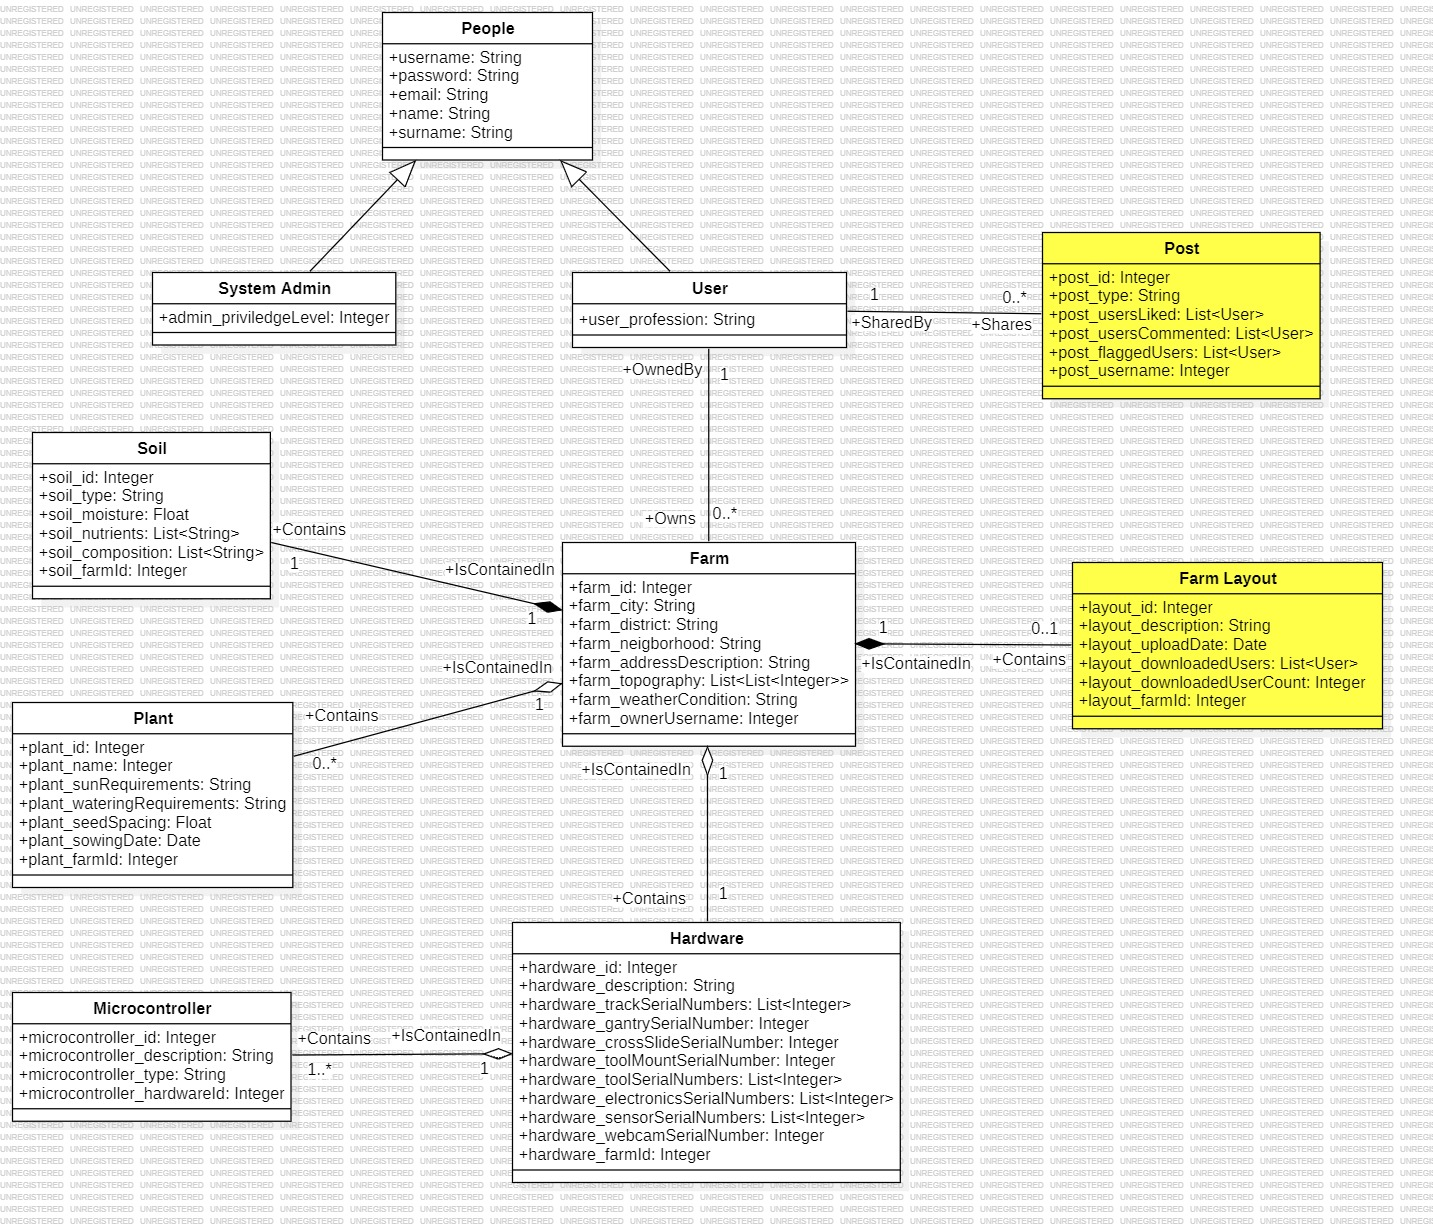
\includegraphics[width=1\linewidth]{Figures/improved_logical_database_diagram.jpg}
    \caption{Logical Database Diagram of the Improved System}
    \label{LogicalDatabaseImproved}
\end{figure}

\newpage

\section{Design Constraints}
Introducing the Mobile Application and ForumBot to the FarmBot project brings new design constraints:
\begin{itemize}
    \item \textbf{Mobile App Security \& Compatibility:} The app must be secure and work smoothly on different devices and operating systems by protecting users' information.
    \item \textbf{ForumBot Safety \& Privacy:} ForumBot needs features for safe community interaction, including privacy protection and tools to handle inappropriate content.
    \item \textbf{Content Moderation:} Tools to monitor and manage content are essential to keep ForumBot positive and respectful.
    \item \textbf{Data Sharing:} Sharing and using farm layouts between FarmBot and ForumBot should be straightforward, with common data formats for compatibility.
\end{itemize}
These new constraints aim to make sure FarmBot's expanded features are user-friendly, secure, and accessible to all.

\section{System Quality Attributes}
To enhance the system quality attributes of FarmBot, considering the new additions of the Mobile Application and ForumBot, the following points are integrated:
\begin{itemize}
    \item \textbf{Reliability (ForumBot \& Mobile App):}
    \begin{itemize}
        \item Ensure consistent performance of ForumBot to support community engagement without disruptions.
        \item The Mobile Application should have mechanisms to handle offline scenarios or weak network conditions, ensuring task scheduling and monitoring are always accessible.
    \end{itemize}
    \item \textbf{Availability (ForumBot \& Mobile App):}
    \begin{itemize}
        \item ForumBot should implement failover strategies to maintain its availability for user interactions even during high traffic or server maintenance.
        \item The Mobile Application requires effective synchronization with FarmBot's cloud services to keep user data up-to-date across all platforms.
    \end{itemize}
    \item \textbf{Security (ForumBot \& Mobile App):}
    \begin{itemize}
        \item Secure authentication and encryption for ForumBot and the Mobile Application to protect user interactions and personal information.
        \item Implement additional security measures for ForumBot to prevent spam, abuse, and data breaches within the community platform.
    \end{itemize}
    \item \textbf{Maintainability (ForumBot):}
    \begin{itemize}
        \item Design ForumBot with a scalable architecture to accommodate growing user base and content without compromising performance.
        \item Regular updates and community feedback loops in ForumBot to enhance features and address user needs effectively.
    \end{itemize}
    \item \textbf{Portability (Mobile App):}
    \begin{itemize}
        \item The Mobile Application should be developed with cross-platform frameworks to ensure seamless functionality across iOS, Android, and other mobile operating systems.
    \end{itemize}
\end{itemize}
These additions aim to enhance the quality of FarmBot's ecosystem, ensuring that the new features provide a secure, reliable, and user-friendly experience while accommodating the expanding scope of the project.

\section{Supporting Information}
The FarmBot project has expanded with the Mobile Application and ForumBot. This broadens community engagement and interaction possibilities.
\begin{itemize}
    \item \textbf{Mobile Application:} The FarmBot Mobile Application brings farm management to users' smartphones, allowing them to control their FarmBot from anywhere. Developers can help to improve the app's functionality and design to meet the community's needs.
    \item \textbf{ForumBot:} This platform enables the FarmBot community to exchange knowledge, experiences, and layouts. Users can contribute by posting content, answering questions, and sharing feedback, encouraging a collaborative space for discussion and innovation.
    \item \textbf{Community Contributions:} The introduction of Mobile Application and ForumBot opens new avenues for contributions beyond traditional software development, including community support and educational outreach, enriching the FarmBot ecosystem for users worldwide.
\end{itemize}
Integration of these new features strengthens the FarmBot community's collaborative efforts in advancing sustainable, technology-driven agriculture.